Dans cette section, on va parler de (mais pas de tous les) axiomes définissant la théorie des ensembles. Ces axiomes sont hors programme, mais en avoir entendu parler permet de poser une fondation plus solide sur ce qui est "correct" et ce qui ne l'est pas. En théorie des ensembles, on ne manipule que des ensembles. Quand on quantifie sans précision, par exemple $\forall x$ ou $\exists x$, $x$ est seulement supposé être un ensemble.
Pour des raisons fondamentales à un point contrariant, nous ne pouvons pas donner mieux qu'une définition intuitive de la notion d'ensemble. 

\begin{dftn}
    Un \emph{ensemble} $E$ est une collection d'objets, sans ordre ni multiplicité. On  appelle \emph{éléments} les objets appartenant à $x$. On note $x \in E$ si $x$ est un élément de $E$, et $x \notin E$ autrement.
\end{dftn}

% \begin{ax}
%     Si $E, F$ sont deux ensembles, l'assertion "$E = F$" est vrai si et seulement si $\forall x, x \in E \Leftrightarrow X \in F$.
% \end{ax}

On peut écrire un ensemble de deux façons :
\begin{itemize}
    \item en \emph{extension}, en écrivant tous ses éléments, entre accolades, séparé par des virgules.
    \begin{lined}
        Les ensembles $\{0,1,2\}, \{2,0,1\}$ et $\{2,2,1,0,1\}$ sont le même ensemble. $\{\NN\}$ est également un ensemble. Il n'a qu'un seul élément, on dit que c'est un singleton. $\{\}$, aussi noté $\emptyset$, existe et est l'unique ensemble qui n'a aucun élément. On l'appelle l'\emph{ensemble vide}.
    \end{lined}
    Il est évident qu'il est difficile d'écrire des ensembles trop gros de cette façon.
    \item en \emph{compréhension}, étant donné un ensemble $E$ et un prédicat $P$ défini sur $E$, on peut former $\{x \in E\sepp P(x)\}$, l'ensemble des éléments de $E$ tels que $P(x)$ est vraie. Dans le cas particulier où $f$ est une fonction de $E$ dans $F$, on note plus simplement $\{f(y) \sepp y \in E\}$ plutôt que $\{x \in F \sepp \exists y \in E, x = f(y)\}$.
    \begin{lined}
        $\{2^k \sepp k \in \NN\}$ est l'ensemble des puissances positives de 2. $\{x \in \RR \sepp \cos(x) = 0\}$ est l'ensemble des solutions de l'équation $\cos(x) = 0$.
    \end{lined}
\end{itemize}

La possibilité d'écrire les ensembles de cette façon est assurée par des axiomes, notamment \emph{de la paire} et \emph{de l'union} pour l'extension, et par le \emph{schéma d'axiomes de compréhension} pour la compréhension. Leur définition non ambiguë est affirmée par l'axiome d'\emph{extensionnalité}.

% \begin{ax}[Paire]
%     Si $E, F$ sont des ensembles, il existe un ensemble $G$ tel que $$x \in G \Rightarrow x = E \vee x = F.$$
% \end{ax}

% \begin{ax}[Union]
%     Si $E$ est un ensemble, il existe un ensemble $F$, appelé l'\emph{union} de $E$, noté $\bigcup E$, tel que $$\forall x, x \in F \Leftrightarrow (\exists G \in E, x \in G).$$
% \end{ax}



\begin{dftn}
    On appelle \emph{cardinal} d'un ensemble fini $E$ le nombre de ses éléments. Les notations $|E|$ et $\#E$ sont généralement acceptées pour dénoter le cardinal de $E$.
\end{dftn}

Le prototype de l'ensemble de cardinal $n$, $n \in \NN$ donné, est l'ensemble $\{m \in \NN \sepp 1 \leq n \leq n\}$, noté $\intint{1, n}$. En fait, on le verra plus tard, on définit plus proprement le cardinal d'un ensemble fini $E$ comme étant l'unique entier $n$ tel que $E$ et $\intint{1, n}$ sont en \emph{bijection}.
Plus généralement, pour $a, b$ entiers relatifs avec $a\leq b$, on note $\intint{a, b}$ l'ensemble des entiers entre $a$ et $b$, de cardinal $b-a+1$.

\begin{dftn}
    Soient $E, F$ deux ensembles.
    \begin{itemize}
        \item Si pour tout $x, x \in E$ entraine $x\in F$, on dit que $E$ est inclus dans $F$, ou que $E$ est une \emph{partie} de $F$. On note $E \subset F$.
        \item Deux ensembles sont \emph{égaux} s'ils ont les mêmes éléments : $\forall x \in E, x \in E \Leftrightarrow x \in F$ (assertion dont la vérité  est bien sûr équivalente à celle de $\forall x \in F, x \in E \Leftrightarrow x \in F$). On note $E = F$.
    \end{itemize}
\end{dftn}

"\^Etre inclus" est, comme $=$, un prédicat binaire. Étant donné trois ensembles $A, B, C$, l'assertion $A \subset B \subset C$, évaluée "naturellement" de la gauche vers la droite, n'a \emph{a priori} pas de sens. Cependant, pour signifier $(A \subset B)\wedge(B \subset C)$, on commet l'abus de notation $A \subset B \subset C$.

\begin{lined}
    Pour tout ensemble $E$, $\emptyset \subset E$. En effet, $\forall x \in \emptyset, x\in E$.
\end{lined}

Il est également clair que $E = F \Leftrightarrow E \subset F \wedge F \subset F$. Ainsi, pour montrer l'égalité de deux ensemble on raisonne souvent par  \emph{double inclusion} plutôt qu'en montrant qu'un objet est dans le premier ensemble si et seulement si il est dans le second. Les deux modes de raisonnement sont néanmoins valides : comme partout on choisit celui qui rend la démonstration agréable.

\begin{rlined}
    Attention, être inclus et être un élément n'est pas \emph{du tout} la même chose. L'ensemble vide est inclus dans $\{1, 2, 3\}$, mais n'en est pas un élément. De même $\pi \in \RR$, mais $\{\pi\} \notin \RR$. Dans la même veine, $\{3\}$ n'est pas la solution de l'équation $x = 3$, mais l'\emph{ensemble de ses solutions}.
\end{rlined}

\begin{ax}
    Si $E$ est un ensemble, il existe un ensemble $F$ tel que $x \in F \Leftrightarrow x \subset E$. On l'appelle l'\emph{ensemble des parties} de $E$ et on le note $\mathfrak{P}(E)$, ou parfois $2^E$.
\end{ax}

\begin{lined}
    L'ensemble des parties $\{1, 2, 3\}$ est $\{\emptyset, \{1\}, \{2\}, \{3\}, \{1, 2\}, \{2, 3\}, \{1, 2\}, \{1, 2, 3\}\}$.
\end{lined}

\subsection{Opérations sur les ensembles.}

\begin{dftn}
    Soient $E$ et $F$ deux ensembles. Il existe un ensemble $G$, noté $E \cup F$, appelé l'\emph{union} de $E$ et $F$, tel que $\forall x, x \in G \Leftrightarrow (x \in E \vee x \in F)$.
    
    Si $(E_i)_{i\in I}$ est une famille (possiblement infinie) d'ensembles indexée par un ensemble $I$, il existe un ensemble $G$ vérifiant $\forall x, x\in G \Leftrightarrow \exists i \in I, x\in E_i$. On note $\bigcup_{i\in I} E_i$ cette union.
\end{dftn}

On donne ici l'union d'une famille d'ensemble comme définition, mais en fait, l'existence de l'ensemble union est axiomatique (elle est affirmée par le bien nommé \emph{axiome de l'union}). En général, on ne peut pas démontrer que cette union existe à partir de rien, on \emph{décide} qu'elle existe.

\begin{dftn}
    Soient $E$ et $F$ deux ensembles. L'ensemble $\{x \in E \sepp x \in F\}$ (ou, de façon équivalente $\{x \in F \sepp x \in E\}$) est noté $E \cap F$ et est appelée l'\emph{intersection} de $E$ et $F$. 
        
    On note $\bigcap_{i \in I} E_i$ l'intersection d'une famille (possiblement infinie) d'ensembles indexée par un ensemble $I$, c'est-à-dire l'ensemble $\{x \in \bigcup_{i\in I}E_i \sepp \forall i \in I, x \in I\}$.
\end{dftn}

Pourquoi ce bizarre "$x \in \bigcup_{i\in I}E_i$" dans l'expression de l'intersection ? Parce que lorsqu'on écrit un ensemble en compréhension, il faut préciser d'où on tire les éléments et comme l'intersection est toujours incluse dans l'union (s'en convaincre), on peut les tirer de l'union. Comme on a également $\forall j \in I$, $\bigcap_{i\in I}E_i \subset E_j$, on aurait pu aussi choisir un des $E_i$ et prendre les $x$ dedans... si on accepte l'axiome \emph{du choix}\footnote{et on l'accepte !}.

\begin{rlined}
    \begin{exo}
        Montrer que pour tous ensembles $A, B$, $A \subset B \Leftrightarrow A \cap B = A$ et que $A \subset B \Leftrightarrow A \cup B = B$
    \end{exo}
\end{rlined}

\begin{dftn}
    Soient $E, F$ deux ensembles.
    \begin{itemize}
        \item L'ensemble $\{x \in E \sepp x \notin F\} \cup \{x \in F \sepp x \notin E\}$ est appelé la \emph{différence symétrique} de $E$ et $F$. On la note $E \Delta F$.
        \item Supposons que $E \subset F$. Le \emph{complément} de $E$ dans $F$ est l'ensemble $\{x \in F \sepp x \notin E\}$. On le note $F \setminus E$ (lire dans ce cas "$F$ privé de $E$") ou $\complement_F^E$. Si l'identité de $F$ est claire en contexte, on note parfois aussi $\overline{E}$.
    \end{itemize}
\end{dftn}

Pour le plus grand malheur des mathématiciens de tous âges, on n'a pas beaucoup de symboles vraiment différents et faciles à écrire. Ainsi, on trouve souvent écrit $F \setminus E = \{x \in F \sepp x \notin E\}$, \emph{sans l'hypothèse que $E \subset F$}. On appelle cela le \emph{complémentaire relatif} de $E$ dans $F$. Dans la suite de ce chapitre, on ne parlera de complémentaire que dans le cas d'inclusion. Heureusement, comme pour tous ensembles $E, F$ on a $F \setminus E = F \setminus (F \cap E)$, il est facile de passer d'un cas à l'autre.

\begin{rlined}
    \begin{exo}
        Montrer que $\forall E, \forall F, E\Delta F = F\Delta E$.
    \end{exo}
    \begin{exo}
        Soient $E, F$ des sous-ensembles d'un ensemble $G$. Montrer que $$(E \cap F = \emptyset \wedge E \cup F = G) \Rightarrow E = \overline{F}.$$
    \end{exo}
\end{rlined}

\begin{dftn}
    \begin{itemize}
        \item Soient $E, F$ des ensembles. Si $E \cap F = \emptyset$, on dit qu'ils sont \emph{disjoints}. On dit que leur union est une \emph{union disjointe} et on le signifie en notant $E \sqcup F$. De même, si une famille $(E_i)_{i\in I}$ indexée par un ensemble $I$ vérifie
        $$\forall i \in I, \forall j \in I, i \neq j, E_i \cap E_j = \emptyset,$$
        on note leur union $\bigsqcup_{i\in I}E_i$.
        \item Soit $F$ un ensemble et $(E_i)_{i\in I}$ une famille d'ensembles indexée par un ensemble $I$ telle que $F = \bigsqcup_{i\in I}E_i$. On dit que la famille $(E_i)_{i\in I}$ est un \emph{recouvrement disjoint} de $F$. Sous l'hypothèse supplémentaire qu'aucun des $E_i$ n'est vide, on parle de \emph{partition} de $F$.
    \end{itemize}
\end{dftn}

\begin{lined}
    Par exemple, $\{E \in \mathfrak{P}(\NN) \sepp \#E = 1\}$ est une partition de $\NN$. \'Etant donné un ensemble fini $E$ de cardinal $n$, $\{\{F \subset E \sepp \#F = k\} \sepp k \in \intint{0, n}\}$ est une partition de $\mathfrak{P}(E)$.
\end{lined}

\newpage

\subsection{Lien avec la logique et compatibilité des opérations.}
\label{sets_log}

Il ne vous aura pas échappé que les opérations ensemblistes ont un comportement suspicieusement similaire à celui de la logique booléenne, au point où l'on note le complément et la négation de la même façon. Voyons les correspondances avec les autres connecteurs logiques.

Dans ce paragraphe \ref{sets_log}, $E,F,G$ désignent, une bonne fois pour toutes, des ensembles. On suppose également que $E, F$ sont des sous-ensembles de $G$. On y note $x$ un élément quelconque de $G$.

\begin{table}[h!]
    \begin{tblr}{X[c,m]X[c,m]X[c,m]X[2,c,m]}
        \textsc{Opération ensembliste} & \textsc{Propriété définissant les éléments} & \textsc{Opération logique correspondante} & \textsc{Patates}\\
        \hline\hline
        $E \cap F$ & $x \in E \wedge x \in F$ & $\wedge$ & 
        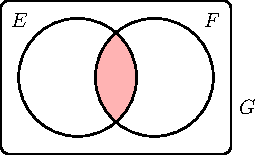
\includegraphics[align = c]{./figures/cap.pdf}\\
        $E \cup F$ & $x \in E \vee x \in F$ & $\vee$ & 
        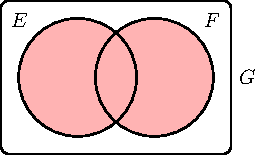
\includegraphics[align = c]{./figures/cup.pdf}\\
        $G \setminus F$ & $\neg(x \in F)$ & $\neg$ (presque) & 
        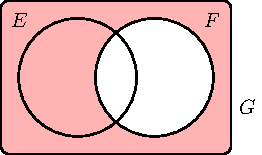
\includegraphics[align = c]{./figures/neg.pdf}\\
        $E \Delta F$ & $x \in E \oplus x \in F$ & $\oplus$ (ou exclusif) & 
        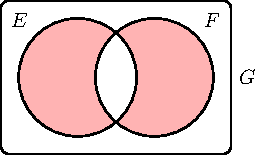
\includegraphics[align = c]{./figures/xor.pdf}\\
        $G \setminus (E \Delta F)$ & $x \in E \Leftrightarrow x \in F$ & $\Leftrightarrow$ & 
        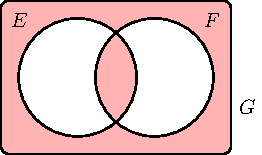
\includegraphics[align = c]{./figures/equiv.pdf}\\
    \end{tblr}
    \caption{Correspondance entre opérateurs logiques et opérations ensemblistes.}
    \label{tab:log=ens}
\end{table}

\newpage

Notons que, contrairement au cas de la logique "pure", on a besoin d'un contexte pour le complémentaire : $\NN \setminus \{1, 2, 3\}$ existe, mais l'ensemble contenant tous les objets possibles sauf ceux de $\{1, 2, 3\}$ n'existe pas. En contraste, le prédicat $\notin \{1,2,3\}$ est bien défini pour tous les objets (on peut toujours, au moins en théorie, tester l'appartenance à un ensemble). Si on choisit de se restreindre au cas, souvent suffisant, où le prédicat est défini sur un ensemble, les deux notions redeviennent équivalentes.

On peut également voir l'implication comme une assertion ensembliste : si $P$ et $Q$ sont des prédicats définis sur $G$, $P$ implique $Q$, si et seulement si $\{x \in G \sepp P(x)\} \subset \{x \in G \sepp Q(x)\}$. Ainsi, le raisonnement par double inclusion est l'analogue ensembliste du raisonnement par double implication.

\begin{rlined}
    \begin{exo}[\textsc{Fait en cours}]
        Soient $a, b$ des réels tels que $a \leq b$. Montrer que $[a, b] = \{ta+(1-t)b\sepp t \in [0, 1]\}$. 
    \end{exo}
    \begin{exo}[\textsc{Important}]
        Montrer les propriétés suivantes.
        \begin{itemize}
            \item $E \cap \emptyset = \emptyset, E\cup\emptyset = E, E\cap G = E, E\cup G = G$.
            \item $E \cap F = F \cap E$ et $E \cup F = F \cup E$.
            \item $(E \cap F) \cap G = E \cap (F \cap G)$ et $(E \cup F) \cup G = E \cup (F \cup G)$.
            \item $(E \cap F) \cup G = (E \cup G) \cap (F \cup G)$ et $(E \cup F) \cap G = (E \cap G) \cup (F \cap G)$.
            \item Si $E \subset G$, $(G \setminus (G \setminus E)) = E$.
            \item Si $E, F$ sont des parties de $G$, $G \setminus (E \cap F) = (G \setminus E) \cup (G \setminus F)$.
            
            et $G \setminus (E \cup F) = (G \setminus E) \cap (G \setminus F)$.
        \end{itemize}
    \end{exo}
\end{rlined}

On doit être capable de montrer formellement ces propositions, mais on peut facilement s'en convaincre par un dessin. Par exemple :
\begin{table}[h!]
    \begin{tblr}{X[c,m]cX[c,m]cX[c,m]}
        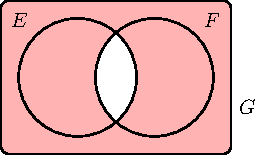
\includegraphics[align = c]{./figures/negcap.pdf} 
        & $=$ & 
        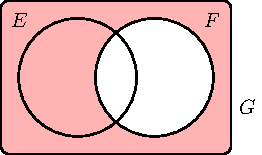
\includegraphics[align = c]{./figures/neg.pdf} 
        & $\cup$ &
        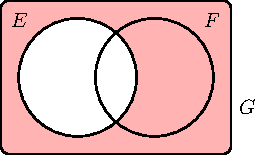
\includegraphics[align = c]{./figures/negF.pdf} \\
    \end{tblr}
\end{table}

Évidemment, ces propriétés s'adaptent quand on fait une intersection ou une union sur une famille quelconque. Prouvons, pour la pratique, la propriété suivante.

\begin{prop}
    Soit $(E_i)_{i\in I}$ une famille d'ensembles indexée par $I$ et $F$ un ensemble. On a $(\bigcap_{i\in I} E_i)\cup F = \bigcap_{i\in I} (E_i \cup F)$.
\end{prop}

\begin{proof}
    Pour tout $x$, on a :
    \begin{align}
        x \in (\bigcap_{i\in I} E_i)\cup F & \Leftrightarrow x \in F \vee (\forall i \in I, x \in E_i)\\
        & \Leftrightarrow \forall i \in I, (x \in F \vee x \in E_i) \\
        & \Leftrightarrow x \in \bigcap_{i\in I} (E_i \cup F)
    \end{align}
\end{proof}

En fait, énervons-nous. Pour nous habituer aux techniques, prouvons la proposition \ref{exo:germain}. Elle n'est pas très utile, mais sa preuve constitue un bon entrainement.
\begin{prop}\label{exo:germain}
    Soit $I$ un ensemble et soient $(E_i)_{i \in I}, (F_i)_{i \in I}$. On a :
    $$\bigcup_{i \in I}(E_i \cap F_i) = \bigcap_{X \in \mathfrak{P}(I)}\left(\bigcup_{i \in X} E_i \cup \bigcup_{i \in I \setminus X} F_i\right).$$
\end{prop}

\begin{proof}
    Faite en cours.
\end{proof}

\subsection{Fonction indicatrice}

Dans ce paragraphe, $E, F, G$ sont des ensemble et $E \subset G$.

\begin{dftn}
   La \emph{fonction indicatrice} de $E$ est la fonction à valeurs réelles, définie sur $G$, notée $\ind_E$, donnée par :
   $$\forall x \in F, f(x) = \left\{\begin{aligned}
    1& \textrm{ si } x \in E\\
    0& \textrm{ sinon}
   \end{aligned}\right.$$
\end{dftn}

\begin{prop}
    \begin{itemize}
        \item $\ind_{G \setminus E} = 1 - \ind_E$.
        \item $\ind_{E \cap F} = \ind_E\cdot\ind_F$.
        \item $\ind_{E \cup F} = \max(\ind_E, \ind_F) = \ind_E + \ind_F - \ind_E \cdot \ind_F$.
    \end{itemize}
\end{prop}

\begin{proof}
    Faite en cours.
\end{proof}

\begin{rlined}
    \begin{exo}
        Utiliser ces propriétés pour générer les tables de vérités de l'exercice \ref{exo:bool} à l'aide d'un tableur (LibreOffice Calc, par exemple).
    \end{exo}
\end{rlined}

\subsection{Produit cartésien}

Considérons deux ensembles $E, F$. On peut écrire, en extension, $\{E\}$ et $\{E, F\}$, puis $\{\{E\}, \{E, F\}\}$. Cette manière de faire a un avantage : on gagne une idée d'ordre entre les parties de $\{\{E\}, \{E, F\}\}$ (l'une est inclus dans l'autre, mais pas réciproquement). 

\begin{dftn}
    Soient $E, F$ deux ensembles. Le \emph{produit cartésien} de $E$ et $F$, noté $E \times F$, est l'ensemble 
    $$\{X \in \mathfrak{P}(\mathfrak{P}(E \cup F)) \sepp \exists x \in E, \exists y \in F, X = \{\{x\}, \{x, y\}\}\}.$$
    On appelle les éléments de $E \times F$ des \emph{couples}. 
\end{dftn}

On peut itérer cette construction et obtenir ainsi des triplets, quadruplets... $n$-uplets pour tout $n$ entier naturel.
Cette construction formelle est hors programme, on demande seulement de connaitre la définition intuitive suivante :

\begin{dftn}
    Soit $n$ un entier supérieur ou égal à 2 et $E_1, E_2, \dots, E_n$ des ensembles. Le \emph{produit cartésien} de $E_1, E_2, \dots, E_n$ est l'ensemble des listes ordonnées $(x_1, x_2, \cdot, x_n)$ avec, pour tout $i \in \intint{1, n}, x_i\in E_i$. On le note $E_1\times E_2 \times ... \times E_n$, ou $E^n$ si tous les $E_i$ sont le même ensemble~$E$.
\end{dftn}

Par convention, on décide que $E^1 = E$ et que $E^0 = \emptyset$.

\begin{figure}[h!]
    \begin{center}
        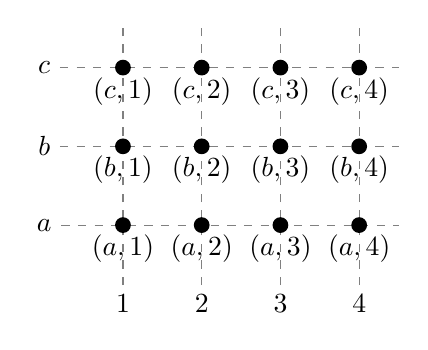
\begin{tikzpicture}
            \node (a) at (-1, 0) {$a$};
            \node (b) at (-1, 1) {$b$};
            \node (c) at (-1, 2) {$c$};
            \node (1) at ( 0,-1) {$1$};
            \node (2) at ( 1,-1) {$2$};
            \node (3) at ( 2,-1) {$3$};
            \node (4) at ( 3,-1) {$4$};

            \draw[dashed, gray] (a) -- (3.5, 0);
            \draw[dashed, gray] (b) -- (3.5, 1);
            \draw[dashed, gray] (c) -- (3.5, 2);
            \draw[dashed, gray] (1) -- ( 0,2.5);
            \draw[dashed, gray] (2) -- ( 1,2.5);
            \draw[dashed, gray] (3) -- ( 2,2.5);
            \draw[dashed, gray] (4) -- ( 3,2.5);

            \fill (0,0) circle (0.1);
            \fill (0,1) circle (0.1);
            \fill (0,2) circle (0.1);
            \fill (1,0) circle (0.1);
            \fill (1,1) circle (0.1);
            \fill (1,2) circle (0.1);
            \fill (2,0) circle (0.1);
            \fill (2,1) circle (0.1);
            \fill (2,2) circle (0.1);
            \fill (3,0) circle (0.1);
            \fill (3,1) circle (0.1);
            \fill (3,2) circle (0.1);

            \node[below] at (0,0) {$(a, 1)$};
            \node[below] at (0,1) {$(b, 1)$};
            \node[below] at (0,2) {$(c, 1)$};
            \node[below] at (1,0) {$(a, 2)$};
            \node[below] at (1,1) {$(b, 2)$};
            \node[below] at (1,2) {$(c, 2)$};
            \node[below] at (2,0) {$(a, 3)$};
            \node[below] at (2,1) {$(b, 3)$};
            \node[below] at (2,2) {$(c, 3)$};
            \node[below] at (3,0) {$(a, 4)$};
            \node[below] at (3,1) {$(b, 4)$};
            \node[below] at (3,2) {$(c, 4)$};

        \end{tikzpicture}
    \end{center}
    \caption{Exemple : produit cartésien de $\{a,b,c\}$ et $\{1,2,3,4\}$.}
\end{figure}
Maintenant que nous connaissons la définition de produit cartésien, on peut définir proprement le terme de "famille indexée par", que l'on a déjà beaucoup utilisée.

\begin{dftn}
    Soit $E, I$ deux ensembles. On appelle \emph{famille indexée par $I$} toute partie $F$ du produit cartésien $I \times E$ tel que pour tout \emph{index} $i$, il existe une unique \emph{valeur} $x \in E$ tel que $(i, e) \in F$.\footnote{En passant, on appelle aussi ça une \emph{fonction} définie sur $I$, mais on en reparlera}
\end{dftn}

La condition signifie simplement qu'il faut que chaque index serve ("pour tout...") et qu'il ne serve qu'une seule fois ("une unique..."). On peut voir ça comme accrocher une petite décoration venue de $I$ aux éléments de $E$ pour ne pas les confondre au cas on voudrait avoir plusieurs fois le même élément (comme des décorations de verre dans une soirée).

\subsection{Quelques notations habituelles}

Les notations précédentes sont en grande partie déjà apparues.

\begin{itemize}
    \item $\NN$ est l'ensemble des nombres entiers naturels.
    \item $\ZZ$ est l'ensemble des nombres entiers relatifs.
    \item $\QQ$ est l'ensemble des nombres rationnels.
    \item $\RR$ est l'ensemble des nombres réels.
    \item $\CC$ est l'ensemble des nombres complexes.
    \item On note $\NN^*, \ZZ^*, \QQ^*, \RR^*, \CC^*$ pour désigner les ensembles précédents privés de $0$. Attention, cette notation est réservée pour ces ensembles spéciaux.
    \item On note $\QQ^+, \QQ^-, \RR^+, \RR^-$ les sous-ensembles des nombres positifs et négatifs de $\QQ$ et $\RR$. On peut aussi note $\QQ^{+*}, \RR^{-*}$... Dans ces derniers cas de figures, on trouve parfois la notation $\QQ_-^*, \RR_+^*$... plus harmonieuse.
    \item Si $a, b \in \RR$, avec $a<b$, on note $[a, b] = \{x \in \RR \sepp a \leq x \leq b\}$. On appelle cet ensemble le \emph{segment} de $a$ à $b$.
    \item Si $a, b \in \RR$, avec $a<b$, on note $]a, b] = \{x \in \RR \sepp a < x \leq b\}$. On appelle cet ensemble l'\emph{intervalle ouvert en $a$, fermé en $b$}. On définit de même $[a, b[$, l'\emph{intervalle fermé en $a$, ouvert en $b$}.
    \item Si $a, b \in \RR$, avec $a<b$, on note $]a, b[ = \{x \in \RR \sepp a < x < b\}$. On appelle cet ensemble l'\emph{intervalle ouvert} de $a$ à $b$.
\end{itemize}